\chapter{IMPLEMENTATION (using MPU-6050)}
\label{chap:MoreStuff}

\section{Implementation}
MPU-6050 was connected to the Wemos board as shown in the above
pin diagram. SCL and SDA pins are used for sending data via I2C
communication protocol.

Using Ardunio IDE we programmed Wemos Board to get accelerometer
and gyroscope data.

Accelerometer data had gravity component in all three axes which is
undesirable and so we filtered that out using a low pass filter by applying
the following transformation on all three axes.
g = 0.9 * g + 0.1 * v
Where g is a global variable initialized to 0 and v is accelerometer reading
of any axis.

7

Using v = v – g you can remove the gravity factor in that axis.
Time interval between two readings was calculated using the difference
in the times in milliseconds returned by the millis() function in the Ardunio
library.

We created a local server using XAMPP and using ESP8266 we uploaded
the MPU data using PHP to MySQL database that was hosted on the local
server.

Once the data was uploaded using the server then the data from the local
server was fetched using python library MySQLdb. We then applied
complementary filters on the raw data to remove noise.

We initially tried to interpolate the accelerometer readings using the
interpolate function in SciPy module. But the results of the plot and time
taken to plot was not at all satisfactory so we then used the Simpson’s
Method of integration using the simps() function in the scipy.integrate
module. Using this we integrated the acceleration data twice with respect
to time to get displacement.

Finally after receiving the displacements in all 3 directions, we used
matplotlib.pyplot to get the 3D graph of the motion.

\section{Problems Faced}
As mentioned above, the MPU-6050 is a cheap module and thus
generates a lot of noise in the data. While, for a lot of applications this
noise can be filtered effectively and the MPU-6050 can be used
satisfactorily, but in our case even the slightest of noise got magnified over
and over again as we integrated over large time intervals.

8
As a result we always got a increasing or decreasing displacement
irrespective of the motion performed because the errors kept on adding
up.

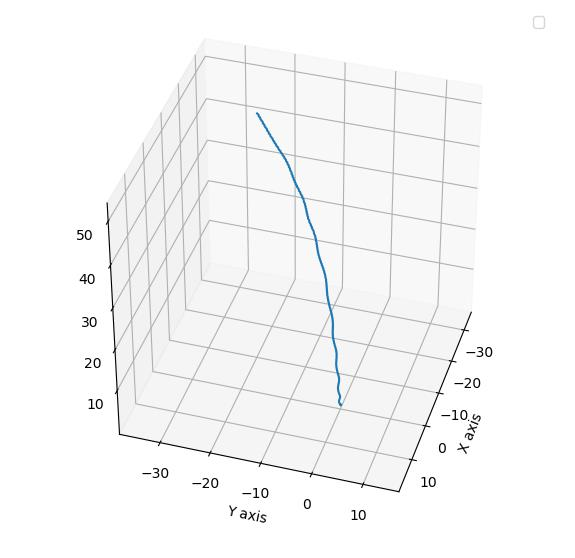
\includegraphics[width=10cm]{plot.png}
